\section{APART Framework}
\label{sec:framework}

In a real-time ride sharing application, the server finds out about a ride and its properties once it receives a request for that ride. At this time, a real-time centralized server has to evaluate the schedule of multiple drivers and decide which driver can best accommodate the new request in its schedule. With a large number of drivers, the scheduling phase soon becomes the bottleneck. In this section we introduce \fname which overcomes this shortcoming by distributing the scheduling process to the drivers themselves. First we explain the auction framework and how the server broadcasts new arriving requests to the drivers. Subsequently, we discuss how each driver generates a bid based on a potential new schedule. We end this section with a discussion on how we can simplify the bid computation process for each driver without sacrificing \fname 's revenue.

\subsection{Request Dispatchment in APART}
\label{subsec:dispatch}

Auction frameworks are simple and allow for a decentralized implementation. For this reason, they have been effectively used for assignment problems \cite{Lagoudakis04,Mehta05}. APART considers drivers as bidders and ride requests as goods. Furthermore, the server plays the role of a central auctioneer in \fname. At a very high level, in \fname, once a new request is received by the server (auctioneer), it presents the request to the drivers (bidders). Each drivers computes a new valid schedule by adding the new request to its current schedule. Based on the new schedule, it generates a bid and submits the bid to the server which represents the profit \fname can make by assigning the request to that driver. The bidding process is performed as a \textit{sealed-bid auction} where drivers simultaneously submit bids and no other driver knows how much the other drivers have bid. The server selects the driver with the highest bid as the winner and matches the request with the driver.

Broadcasting every incoming request to all available drivers incurs a large communication cost on the system. \fname lowers the communication cost by only sending any incoming request to \textit{eligible drivers} that are define as:

\begin{definition} [Eligible Drivers]
An available driver $v$ is said to be eligible for servicing a newly submitted request $r$, if and only if:
\begin{equation*}
distance(v, r.s) \leq r.w \times avg\_speed
\end{equation*}
\end{definition}

\noindent In other words, an available driver \textit{d} is eligible for servicing request \textit{r}, if it has enough time to reach the pick-up location of \textit{r} within \textit{r}'s waiting time. The server maintains a spatial index on the location of the drivers. With Apart, we use a grid index since (1) the drivers have to send updated locations to the server only if they change cells and (2) the server does not need to know the exact location of the drivers to be able to filter out non-eligible workers. For example, in \cref{fig:grid_index}, assuming the black dot is the pick-up location of a new request and $r$ is the maximum wait time for the new request, any driver in the shaded cells will receive the new request.

\begin{figure}[!ht]
	\centering
	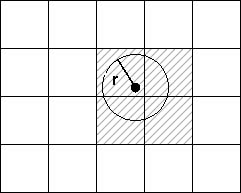
\includegraphics[width=0.45\columnwidth]{fig/grid_index.jpg}
	\vspace{-0mm}\caption{Spatiotemporal Grid Index} \vspace{-2mm} \label{fig:grid_index}
\end{figure}\vspace{-0mm}

\begin{algorithm}
\caption{ALGORITHM($V, r$)}
\label{algo:ALGORITHM}
\begin{algorithmic}[1]
\REQUIRE $V$ is the set of currently available drivers and $r$ is a new request
\ENSURE $v \in V$ as the driver which request $r$ should be assigned to
\STATE $v_{selected} = $ \emph{null}
\STATE $Bids = \emptyset$
\FOR{$v \in V_r$} \label{line:loop_start}
	\STATE $b_v = v$.ComputeBid$(r)$ \label{line:compute}
	\STATE $Bids \leftarrow  b_v$
\ENDFOR \label{line:loop_end}
\STATE $v_{selected} = \argmax_x \left\lbrace b_x \in Bids \right\rbrace$ \label{line:select}
\RETURN $v_{selected}$
\end{algorithmic}
\end{algorithm}

\cref{algo:ALGORITHM} outlines the process of assigning an incoming request $r$. $V_r$ in line \ref{line:loop_start} is the set of eligible drivers for request $r$. Notice that all the iterations of the \textbf{for} loop in \cref{algo:ALGORITHM} (lines \ref{line:loop_start}-\ref{line:loop_end}) run in parallel. The \emph{ComputeBid()} method (line \ref{line:compute}) that each driver executes depends on the bidding rule described in \cref{subsec:bidcomp}. In case of a tie in line \ref{line:select}, the algorithm randomly selects one driver among the ones with the highest bid.

\subsection{Bid Computation \& Payments}
\label{subsec:bidcomp}

With APART, once a driver is notified of a new request, it has to compute a bid. The bid each driver generates reflects the profit the system can make if the request is assigned to that driver. It is important to mention that when discussing the bid computation process for a driver, we are in fact referring to a ride-sharing software on the driver's cell phone. In other words, a ride-sharing application receives the request, generates a bid and submits the bid to the server. Once a diver is assigned a new request, he will be notified with an updated schedule. This means that the human driver's interaction with \fname is limited to configuring his profile on the ride-sharing application\footnote{hereafter, we refer to both the human driver and the software as \textit{driver}.}.

\begin{algorithm}[!h]
\caption{GetProfitAndCost($schedule, start$)}
\label{algo:get_profit}
\begin{algorithmic}[1]
\REQUIRE \emph{schedule} is an ordered list of pick-up/drop-off points and \emph{start} is the current time.
\ENSURE a pair of ($profit, cost$) of performing the input schedule. If the input schedule is not valid it returns ($-\infty, \infty$)
\STATE $time = start$
\STATE $loc = v.$loc\label{ln:loc}
\STATE $trip = 0$
\FOR{$p$ \textbf{in} $schedule$}
	\STATE $path =$ ShortestPath($loc, p$.loc)
	\STATE $trip \pluseq$ Distance($path$)
	\STATE $time \pluseq$ TravelTime($path$)
	\IF{$p$.type $= start$}
		\IF{$time > p$.req.req\_time $+ p$.req.w}
			\RETURN $-\infty$
		\ENDIF
		\STATE $pickUp[p$.req$]=trip$
	\ENDIF
	\IF{$p$.type $= end$}
		\STATE $\delta d = trip - pickUp[p$.req$]$
		\STATE $fare \pluseq p$.f($\delta d$) $\times$ FARE($p$.req.sp)
		\STATE $cost = v$.g($trip$)\label{ln:dprof}
	\ENDIF
\ENDFOR
\STATE $profit = fare - cost$
\RETURN $profit, cost$
\end{algorithmic}
\end{algorithm}

At each point in time, every driver has a schedule $s$. For every request $r_j \in s$, the driver can determine $r_j$'s incurred detour. Subsequently, using \cref{eq:fare,eq:payment,eq:profit} the driver can compute the profit it makes for \fname based on its current schedule, $p_0$. \cref{algo:get_profit} outlines the process of determining the profit each driver can generate based on his current schedule. Each driver $v$ runs this algorithm locally and hence, $v.loc$ (line~\ref{ln:loc}) and $v.g()$ (line~\ref{ln:dprof}) refer to $v$'s current location and profile, respectively. Also, whether $p$ is a pick-up or drop-off point, in \cref{algo:get_proft} $p.req$ refers to the request for which $p$ is one of the end points.

When a driver is notified with a new request $r$, the first step is to find a potential valid schedule that contains every request in it current schedule, $s$, in addition to $r$. If multiple such schedules exist, it chooses the one which generates maximum profit. In order to find a valid schedule, each driver runs a branch and bound algorithm outlined in \cref{algo:can_schedule}. The algorithm is initially called with $f = \emptyset$, $r = s \cup r$, $bp = -\infty$, $bs = \emptyset$ and $start =$ current time. 

\begin{algorithm}[!h]
\caption{CanSchedule($f, r, bp, bs, start$)}
\label{algo:can_schedule}
\begin{algorithmic}[1]
\REQUIRE \emph{f} and \emph{r} are lists of pick-up/drop-off points that have been added and to be added to a valid schedule, respectively. \emph{bp} and \emph{bs} are the best profit and corresponding schedule observed so far and \emph{start} is the current time.
\ENSURE $bp, bs$ as the best profit and corresponding schedule for input points is a valid schedule exists. Otherwise $-\infty, \emptyset$
\IF{$f$.size $+ r$.size $ > v$.n $\times 2$}
	\RETURN $bp, bs$
\ENDIF
\FOR{$p$ \textbf{in} $r$}
	\STATE $f' = f$
	\STATE $f'$.add($p$)
	\STATE $p =$ GetProfit($f', start$)
	\IF{$p \neq -\infty$ and $p \geq bp$}
		\STATE $r' = r$
		\STATE $r'$.remove($p$)
		\IF{$p$.type $= start$}
			\STATE $r'$.add($p$.req.end)
		\ENDIF
		\IF{$r'$.size $= 0$}
			\RETURN $p, f'$
		\ENDIF
		\STATE $p, s =$ CanSchedule($f', r', bp, bs, start$)
		\IF{$p > bp$}
			\STATE $bs = s$
			\STATE $bp = p$
		\ENDIF
	\ENDIF
\ENDFOR
\RETURN $bp, bs$
\end{algorithmic}
\end{algorithm}

Assuming the profit generated from such schedule is $p_m$, the driver can compute its bid, $b_v$, as the \textit{additional profit} it can make for APART by serving $r$. i.e., $b_v = p_m - p_0$, where $p_0$ is the cost of its current schedule. Similarly, $cost_v$ is the additional cost driver $v$ will incur for serving the new request. In other words, if driver $v$'s bid is accepted, he expects a reward equal to $cost_v$ for serving the new request.

Once every driver submits his bid, the server selects the driver with the highest bid as the winner and assigns the new request to him. Assuming driver $v$ wins the auction, his reward for serving the request is the same amount as $cost_v$, based on which he determined the bid value. Also, upon assigning the new request to $v$, the service providers increases its revenue by $b_v$.

%\subsection{Payments in \fname}

%Once every driver submits his bid, the server selects the driver with the highest bid as the winner and allocates the new request to him. Assuming driver $v$ wins the auction with probability $p_v$, his expected compensation is: 

%\begin{equation*}
%E[comp_v] = p_v.Comp_v(win) + (1 - p_v).Comp_v(loose)
%\end{equation*}

%Where $Comp_v()$ gives the compensation driver $v$ receives for winning or loosing the auction. Intuitively, in the case of winning, $v$ gets compensated the same amount as $cost_v$ based on which he determined his bid and receives $\$0$ for loosing, i.e., $E[comp_v] = p_v.cost_v$. We call this payment model first-price, since the compensation the winner receives is only based on the highest bid.

%Earlier we mentioned that the human driver has no interaction with \fname with regard to computing and submitting a bid. However, depending on how the human driver customizes his profile $g()$, he can affect his $cost$ computation and consequently, the bid value~\footnote{Hereafter, when we say the driver increases/decreases his bid, we mean he does it indirectly by customizing his profile}. For example, assume $v_i$ is the winner of the auction with bid $b_i$ and the second highest bid is $b_j$. In theory, if $v_i$ changes his profile such that his bid becomes $b_i - \epsilon (\epsilon < b_i - b_j)$, he will still be the winner of the auction and has gets compensated $\$\epsilon$ more than when his bid was $b_i$. In practice, however, $v_i$ does not know the \textit{actual} value of any other driver's bid. Therefore, for every driver there is a trade-off between lowering the value of the bid and the probability of being the winner. To maximize his compensation, a rational driver makes his bid as close as possible to the \textit{expected} value of the second highest bid. The details of how each driver can compute this expected value is out of the scope of this paper and more details can be found in \cite{Vickery61}.

%In order to facilitate the bid computation process for workers, \fname adopts a payment model in which the drivers do not benefit from increasing/decreasing their cost and bid values. The compensation of the winner driver in \fname is computed as:

%\begin{equation*}
%comp_i = cost_i + (bid_i - bid_j)
%\end{equation*}

%\noindent Where $v_i$ is the driver with the highest bid and $v_j$ is the driver with the second highest bid. Since the compensation depends on not only the highest bid but also the second highest bid, we call it the second-price model. Following we first prove that with the second-price model, each driver can maximize his compensation by configuring their profiles such that it results in the \textit{minimum} cost that is economical for him to participate in the system. Next we show that in the second-price payment model, not only we get the same rider to driver assignments, but also the final revenue of \fname in both model remains the same.

%\begin{theorem}
%In the second-price payment model, a driver has no incentive to configure his profiles such that his resulting cost is either lower or higher than his minimum cost.
%\end{theorem}

%\begin{theorem}
%Both the first-price and second-price payment model result in the same rider to driver assignment and generate the same revenue.
%\end{theorem}